\documentclass{../../slides-style}

\slidetitle[Часть 2]{Веб-программирование}{30.11.2022}

\begin{document}

    \begin{frame}[plain]
        \titlepage
    \end{frame}

    \section{Введение}

    \begin{frame}
        \frametitle{Попробуем написать что-нибудь ``настоящее''}
        \begin{itemize}
            \item Приложение для регистрации на конференцию
            \item Титульная страница конференции со ссылкой на форму регистрации
            \item Форма регистрации
            \begin{itemize}
                \item Как слушатель или как докладчик
            \end{itemize}
            \item Страница, на которой можно просмотреть всех зарегистрировавшихся
            \item Итого, многостраничное приложение на Razor Pages
            \item Create a new project -> ASP.NET Core Web App
        \end{itemize}
    \end{frame}

    \section{Hello, world}

    \begin{frame}[fragile]
        \frametitle{Вид}
        \begin{minted}{html}
@page

<!DOCTYPE html>

<html>
    <head>
        <meta name="viewport" content="width=device-width" />
        <title>Hello</title>
    </head>
    <body>
        Hello, world!
    </body>
</html>
        \end{minted}
    \end{frame}

    \section{Регистрация}

    \begin{frame}[fragile]
        \frametitle{Моделирование данных}
        \begin{minted}{csharp}
namespace ConferenceRegistration.Pages;

[BindProperties]
public class RegistrationModel : PageModel
{
    public string Name { get; set; } = "";

    public string Email { get; set; } = "";

    public bool IsSpeaker { get; set; }
}
        \end{minted}
    \end{frame}

    \begin{frame}[fragile]
        \frametitle{Страница регистрации}
        \begin{ssmall}
            \begin{minted}{html}
@page
@model ConferenceRegistration.Pages.RegistrationModel
@addTagHelper *, Microsoft.AspNetCore.Mvc.TagHelpers

<html>
    <head>
        <meta name="viewport" content="width=device-width" />
        <title>Register</title>
    </head>
    <body>
        <form asp-action="Register" method="post">
            <p>
                <label asp-for="Name">Your name:</label>
                <input asp-for="Name" />
            </p>
            <p>
                <label asp-for="Email">Your email:</label>
                <input asp-for="Email" />
            </p>
            <p>
                <label>Are you a speaker?</label>
                <select asp-for="IsSpeaker">
                    <option value="">Choose an option</option>
                    <option value="true">Yes</option>
                    <option value="false">No</option>
                </select>
            </p>
            <button type="submit">Register!</button>
        </form>
    </body>
</html>
            \end{minted}
        \end{ssmall}
    \end{frame}

    \begin{frame}[fragile]
        \frametitle{Титульная страница}
        \begin{footnotesize}
            \begin{minted}{html}
@page

@addTagHelper *, Microsoft.AspNetCore.Mvc.TagHelpers

<html>
    <head>
        <meta name="viewport" content="width=device-width" />
        <title>SEIM-2023 registration</title>
    </head>
    <body>
        <div>
            <p>SEIM-2023 conference will be (likely) held in April in St. Petersburg.</p>
            <a asp-page="Registration">Register now!</a>
        </div>
    </body>
</html>
            \end{minted}
        \end{footnotesize}
    \end{frame}

    \begin{frame}[fragile]
        \frametitle{Вернёмся к странице регистрации}
        \begin{footnotesize}
            \begin{minted}{csharp}
namespace ConferenceRegistration.Pages;

[BindProperties]
public class RegistrationModel : PageModel
{
    public string Name { get; set; } = "";

    public string Email { get; set; } = "";

    public bool IsSpeaker { get; set; }

    public void OnPost()
    {
        // TODO: Do something with registration info.
    }
}
            \end{minted}
        \end{footnotesize}
    \end{frame}

    \section{Персистентность}

    \begin{frame}[fragile]
        \frametitle{Работа с базой}
        \framesubtitle{Модель данных, Data.Participant.cs}
        \begin{footnotesize}
            \begin{minted}{csharp}
namespace ConferenceRegistration.Data;

public class Participant
{
    public string Name { get; set; } = "";

    public string Email { get; set; } = "";

    public bool IsSpeaker { get; set; }
}
            \end{minted}
        \end{footnotesize}
    \end{frame}

    \begin{frame}[fragile]
        \frametitle{Обновим модель}
        \begin{footnotesize}
            \begin{minted}{csharp}
namespace ConferenceRegistration.Pages;

using ConferenceRegistration.Data;

[BindProperties]
public class RegistrationModel : PageModel
{
    public Participant Participant { get; set; } = new();

    public void OnPost()
    {
        // TODO: Do something with registration info.
    }
}
            \end{minted}
        \end{footnotesize}
    \end{frame}

    \begin{frame}[fragile]
        \frametitle{И представление}
        \begin{ssmall}
            \begin{minted}{html}
@page
@model ConferenceRegistration.Pages.RegistrationModel
@addTagHelper *, Microsoft.AspNetCore.Mvc.TagHelpers

<html>
    <head>
        <meta name="viewport" content="width=device-width" />
        <title>Register</title>
    </head>
    <body>
        <form asp-action="Register" method="post">
            <p>
                <label asp-for="Participant.Name">Your name:</label>
                <input asp-for="Participant.Name" />
            </p>
            <p>
                <label asp-for="Participant.Email">Your email:</label>
                <input asp-for="Participant.Email" />
            </p>
            <p>
                <label>Are you a speaker?</label>
                <select asp-for="Participant.IsSpeaker">
                    <option value="">Choose an option</option>
                    <option value="true">Yes</option>
                    <option value="false">No</option>
                </select>
            </p>
            <button type="submit">Register!</button>
        </form>
    </body>
</html>
            \end{minted}
        \end{ssmall}
    \end{frame}

    \begin{frame}[fragile]
        \frametitle{DbContext}
        \begin{footnotesize}
            \begin{minted}{csharp}
namespace ConferenceRegistration.Data;

using Microsoft.EntityFrameworkCore;

public class ConferenceRegistrationDbContext: DbContext
{
    public ConferenceRegistrationDbContext(
        DbContextOptions<ConferenceRegistrationDbContext> options)
        : base(options)
    {
    }

    public DbSet<Participant> Participants => Set<Participant>();
}
            \end{minted}
        \end{footnotesize}
    \end{frame}

    \begin{frame}[fragile]
        \frametitle{Модель с DbContext}
        \begin{scriptsize}
            \begin{minted}{csharp}
namespace ConferenceRegistration.Pages;
using ConferenceRegistration.Data;

[BindProperties]
public class RegistrationModel : PageModel
{
    private readonly ConferenceRegistrationDbContext _context;

    public RegistrationModel(ConferenceRegistrationDbContext context)
        => _context = context;

    public Participant Participant { get; set; } = new();

    public async Task<IActionResult> OnPostAsync()
    {
        _context.Participants.Add(Participant);
        await _context.SaveChangesAsync();

        return RedirectToPage("./Index");
    }
}
            \end{minted}
        \end{scriptsize}
    \end{frame}

    \begin{frame}[fragile]
        \frametitle{Конфигурация базы}
        \begin{footnotesize}
            \begin{minted}{csharp}
global using Microsoft.AspNetCore.Mvc;
global using Microsoft.AspNetCore.Mvc.RazorPages;

using ConferenceRegistration.Data;
using Microsoft.EntityFrameworkCore;

var builder = WebApplication.CreateBuilder(args);

// Add services to the container.
builder.Services.AddRazorPages();

builder.Services.AddDbContext<ConferenceRegistrationDbContext>(options =>
    options.UseSqlite("Data Source=conferenceRegistration.db"));

var app = builder.Build();
            \end{minted}
        \end{footnotesize}
    \end{frame}

    \begin{frame}[fragile]
        \frametitle{Добавим первичный ключ в модель данных}
        \begin{footnotesize}
            \begin{minted}{csharp}
namespace ConferenceRegistration.Data;

public class Participant
{
    public int ParticipantId { get; set; }

    public string Name { get; set; } = "";

    public string Email { get; set; } = "";

    public bool IsSpeaker { get; set; }
}
            \end{minted}
        \end{footnotesize}
    \end{frame}

    \begin{frame}[fragile]
        \frametitle{Миграции}
        \begin{itemize}
            \item \emph{Миграции} --- механизм обеспечения эволюции схемы БД
            \item Генерируются автоматически по коду
            \item \mintinline{text}{dotnet tool install --global dotnet-ef}
            \item \mintinline{text}{dotnet add package Microsoft.EntityFrameworkCore.Design}
            \item \mintinline{text}{dotnet ef migrations add InitialCreate}
            \item \mintinline{text}{dotnet ef database update}
            \item Последний шаг надо применять каждый раз при создании базы
        \end{itemize}
    \end{frame}

    \section{Остальная функциональность}

    \begin{frame}[fragile]
        \frametitle{Список участников}
        \framesubtitle{ListParticipants.cshtml}
        \begin{ssmall}
            \begin{minted}{html}
@page
@model ConferenceRegistration.Pages.ListParticipantsModel

<html>
    <head>
        <meta name="viewport" content="width=device-width" />
        <title>ListParticipants</title>
    </head>
    <body>
    <h2>List of conference participants:</h2>
    <table>
        <thead>
            <tr>
                <th>Name</th>
                <th>Email</th>
                <th>Is speaker</th>
            </tr>
        </thead>
        <tbody>
            @foreach (ConferenceRegistration.Data.Participant p in Model.Participants) {
                <tr>
                    <td>@p.Name</td>
                    <td>@p.Email</td>
                    <td>@(p.IsSpeaker ? "Yes" : "No")</td>
                </tr>
            }
        </tbody>
    </table>
    </body>
</html>
            \end{minted}
        \end{ssmall}
    \end{frame}

    \begin{frame}[fragile]
        \frametitle{Модель}
        \begin{footnotesize}
            \begin{minted}{csharp}
namespace ConferenceRegistration.Pages;
using ConferenceRegistration.Data;

public class ListParticipantsModel : PageModel
{
    private readonly ConferenceRegistrationDbContext context;

    public ListParticipantsModel(ConferenceRegistrationDbContext context)
        => this.context = context;

    public IList<Participant> Participants { get; private set; } = new List<Participant>();

    public void OnGet()
    {
        Participants = context.Participants.OrderBy(p => p.ParticipantId).ToList();
    }
}
            \end{minted}
        \end{footnotesize}
    \end{frame}

    \begin{frame}[fragile]
        \frametitle{Страница подтверждения регистрации}
        \framesubtitle{Thanks.cshtml}
        \begin{scriptsize}
            \begin{minted}{html}
@page
@model ConferenceRegistration.Pages.ThanksModel

<html>
    <head>
        <meta name="viewport" content="width=device-width" />
        <title>Thanks</title>
    </head>
    <body>
        <p>
            <h1>Thank you, @Model.Participant.Name</h1>
        </p>
        <p>
            @if (Model.Participant.IsSpeaker)
            {
                @:Please don't forget to submit your article!
            }
        </p>
    </body>
</html>
            \end{minted}
        \end{scriptsize}
    \end{frame}

    \begin{frame}[fragile]
        \frametitle{И модель для неё}
        \begin{footnotesize}
            \begin{minted}{csharp}
namespace ConferenceRegistration.Pages;
using ConferenceRegistration.Data;

public class ThanksModel : PageModel
{
    public Participant Participant { get; set; } = new();

    public void OnGet(Participant participant)
    {
        Participant = participant;
    }
}
            \end{minted}
        \end{footnotesize}
    \end{frame}

    \begin{frame}[fragile]
        \frametitle{И редирект на страницу}
        \begin{footnotesize}
            \begin{minted}{csharp}
...
public class RegistrationModel : PageModel
{
    ...
    public async Task<IActionResult> OnPostAsync()
    {
        context.Participants.Add(Participant);
        await context.SaveChangesAsync();

        return RedirectToPage("./Thanks", Participant);
    }
}
            \end{minted}
        \end{footnotesize}
    \end{frame}

    \section{Оформление}

    \begin{frame}[fragile]
        \frametitle{Оформление}
        \framesubtitle{Bootstrap}
        \begin{scriptsize}
            \begin{minted}{html}
@page
@addTagHelper *, Microsoft.AspNetCore.Mvc.TagHelpers

<html>
    <head>
        <meta name="viewport" content="width=device-width" />
        <title>SEIM-2022 registration</title>
        <link rel="stylesheet" href="/lib/bootstrap/dist/css/bootstrap.css" />
    </head>
    <body>
        <div class="text-center">
            <h3>SEIM-2022 conference will be held in April in St. Petersburg.</h3>
            <a class="btn btn-primary" asp-page="Registration">Register now!</a>
        </div>
    </body>
</html>
            \end{minted}
        \end{scriptsize}
    \end{frame}

    \begin{frame}[fragile]
        \frametitle{Форма регистрации}
        \framesubtitle{Лейауты}
        \begin{ssmall}
            \begin{minted}{html}
<div class="row mb-3 text-center"><h4 class="col-sm-6">Registration form</h4></div>
<form asp-action="Register" method="post">
    <div class="row mb-3">
        <label class="col-sm-1 col-form-label col-form-label-lg" 
            asp-for="Participant.Name">Your name:</label>
        <div class="col-sm-4">
            <input class="form-control form-control-lg" 
                asp-for="Participant.Name" />
        </div>
    </div>
    <div class="row mb-3">
        <label class="col-sm-1 col-form-label col-form-label-lg" 
            asp-for="Participant.Email">Your email:</label>
        <div class="col-sm-4">
            <input class="form-control form-control-lg" 
                asp-for="Participant.Email" />
        </div>
    </div>
    ...
    <div class="row mb-3 mx-auto">
        <div class="col-sm-5 d-grid gap-2">
            <button class="btn btn-primary btn-lg" type="submit">
                Register!
            </button>
        </div>
    </div>
</form>
            \end{minted}
        \end{ssmall}
    \end{frame}

    \begin{frame}[fragile]
        \frametitle{Список участников}
        \begin{ssmall}
            \begin{minted}{html}
@page
@model ConferenceRegistration.Pages.ListParticipantsModel

<html>
    <head>
        <meta name="viewport" content="width=device-width" />
        <title>ListParticipants</title>
        <link rel="stylesheet" href="/lib/bootstrap/dist/css/bootstrap.css" />
    </head>
    <body>
        <div class="row mb-3 text-center"><h2 class="col-sm-6">List of conference participants</h2></div>
        <table class="table table-striped table-bordered">
            <thead>
                <tr>
                    <th>Name</th>
                    <th>Email</th>
                    <th>Is speaker</th>
                </tr>
            </thead>
            <tbody>
            @foreach (ConferenceRegistration.Data.Participant p in Model.Participants) {
                <tr>
                    <td>@p.Name</td>
                    <td>@p.Email</td>
                    <td>@(p.IsSpeaker ? "Yes" : "No")</td>
                </tr>
            }
            </tbody>
        </table>
    </body>
</html>
            \end{minted}
        \end{ssmall}
    \end{frame}

    \section{Валидация}

    \begin{frame}[fragile]
        \frametitle{Декларативная валидация}
        \begin{footnotesize}
            \begin{minted}{csharp}
namespace ConferenceRegistration.Data;
using System.ComponentModel.DataAnnotations;

public class Participant
{
    public int ParticipantId { get; set; }

    [Required(ErrorMessage = "Please enter your name")]
    public string Name { get; set; }

    [Required(ErrorMessage = "Please enter your email")]
    [RegularExpression(".+\\@.+\\..+", ErrorMessage = 
        "Please enter a valid email address")]
    public string Email { get; set; }

    [Required(ErrorMessage = 
        "Please specify whether you'll be a speaker or just attending")]
    public bool? IsSpeaker { get; set; }
}
            \end{minted}
        \end{footnotesize}
    \end{frame}

    \begin{frame}[fragile]
        \frametitle{Модель}
        \begin{footnotesize}
            \begin{minted}{csharp}
...
public class RegistrationModel : PageModel
{
    ...
    public async Task<IActionResult> OnPostAsync()
    {
        if (!ModelState.IsValid)
        {
            return Page();
        }

        context.Participants.Add(Participant);
        await context.SaveChangesAsync();

        return RedirectToPage("./Thanks", Participant);
    }
}
            \end{minted}
        \end{footnotesize}
    \end{frame}

    \begin{frame}[fragile]
        \frametitle{Представление}
        \begin{ssmall}
            \begin{minted}{html}
...
<div class="row mb-3 text-center"><h4 class="col-sm-6">Registration form</h4></div>
<form asp-action="Register" method="post">
    <div class="row mb-3">
        <span asp-validation-for="Participant.Name" class="text-danger"></span>
        ...
    </div>
    <div class="row mb-3">
        <span asp-validation-for="Participant.Email" class="text-danger"></span>
        ...
    </div>
    <div class="row mb-3">
        <span asp-validation-for="Participant.IsSpeaker" class="text-danger"></span>
        ...
    </div>
    <div class="row mb-3 mx-auto">
        <div class="col-sm-5 d-grid gap-2">
            <button class="btn btn-primary btn-lg" type="submit">
                Register!
            </button>
        </div>
    </div>
</form>
...
            \end{minted}
        \end{ssmall}
    \end{frame}

    \begin{frame}[fragile]
        \frametitle{Client-side-валидация}
        \begin{scriptsize}
            \begin{minted}{html}
...
<head>
    <meta name="viewport" content="width=device-width" />
    <title>Register</title>
    <link rel="stylesheet" href="/lib/bootstrap/dist/css/bootstrap.css" />
    <script src="/lib/jquery/dist/jquery.js"></script>
    <script src="/lib/jquery-validation/dist/jquery.validate.js"></script>
    <script src="/lib/jquery-validation-unobtrusive/jquery.validate.unobtrusive.js">
    </script>
</head>
...
            \end{minted}
        \end{scriptsize}
    \end{frame}

    \section{Деплой}

    \begin{frame}
        \frametitle{Docker}
        \begin{itemize}
            \item Средство для ``упаковки'' приложений в изолированные контейнеры
            \item Что-то вроде легковесной виртуальной машины
            \item DSL для описания образов 
            \item Публичный репозиторий
            \item Стандарт де-факто для деплоя веб-приложений
        \end{itemize}
        \begin{center}
            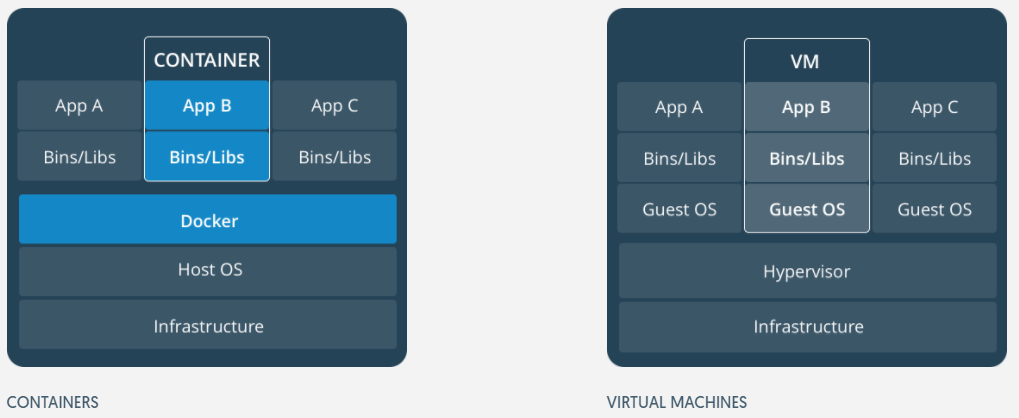
\includegraphics[width=0.7\textwidth]{docker.png}
            \attribution{\url{https://www.docker.com}}
        \end{center}
    \end{frame}

    \begin{frame}
        \frametitle{Docker Image}
        \begin{columns}
            \begin{column}{0.6\textwidth}
                \begin{itemize}
                    \item Окружение и приложение
                    \item Состоит из слоёв
                    \begin{itemize}
                        \item Все слои read-only
                        \item Образы делят слои между собой как процессы делят динамические библиотеки
                    \end{itemize}
                    \item На основе одного образа можно создать другой
                \end{itemize}
            \end{column}
            \begin{column}{0.4\textwidth}
                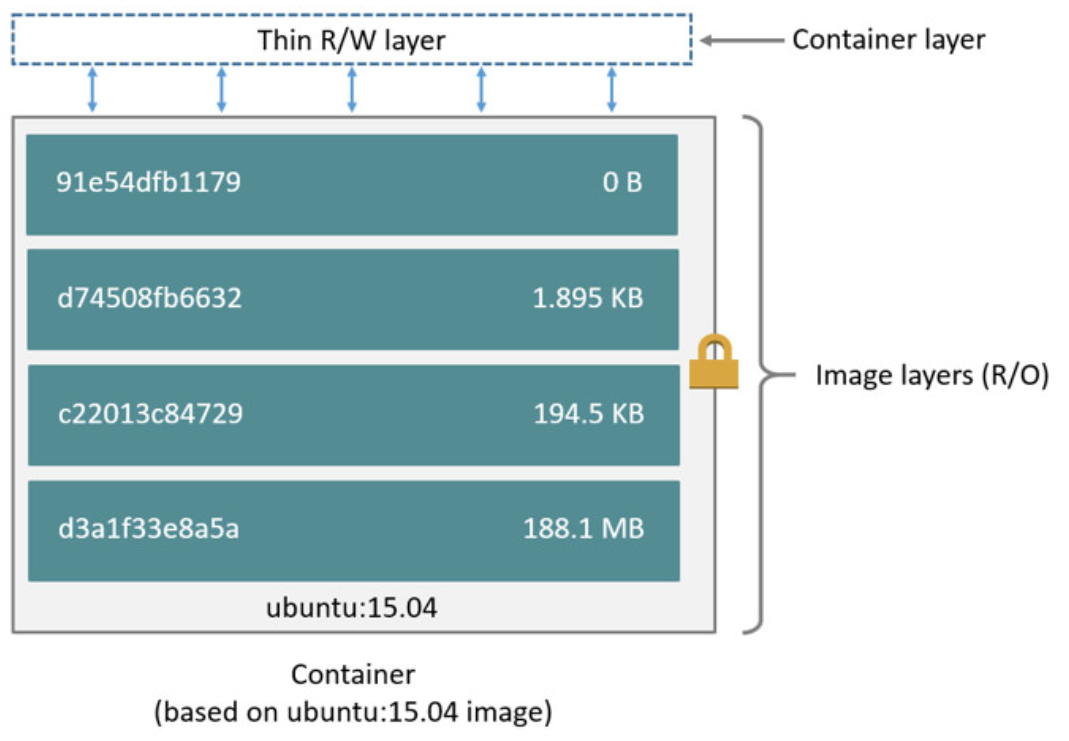
\includegraphics[width=0.9\textwidth]{dockerLayers.png}
            \end{column}
        \end{columns}
    \end{frame}

    \begin{frame}[fragile]
        \frametitle{Dockerfile}
        \begin{scriptsize}
            \begin{minted}{html}
FROM mcr.microsoft.com/dotnet/aspnet:7.0 AS base
WORKDIR /app
EXPOSE 80
EXPOSE 443

FROM mcr.microsoft.com/dotnet/sdk:7.0 AS build
WORKDIR /src
COPY ["ConferenceRegistration.csproj", "."]
RUN dotnet restore "./ConferenceRegistration.csproj"
COPY . .
WORKDIR "/src/."
RUN dotnet build "ConferenceRegistration.csproj" -c Release -o /app/build

FROM build AS publish
RUN dotnet publish "ConferenceRegistration.csproj" -c Release -o /app/publish /p:UseAppHost=false

FROM base AS final
WORKDIR /app
COPY --from=publish /app/publish .
ENTRYPOINT ["dotnet", "ConferenceRegistration.dll"]
            \end{minted}
        \end{scriptsize}
    \end{frame}

    \begin{frame}[fragile]
        \frametitle{Пушим на Docker Hub}
        \begin{itemize}
            \item Регистрируемся на Docker Hub
            \item docker images ls
            \item docker image tag conferenceregistration:latest <ваш юзернейм на Docker Hub>/conferenceregistration:latest
            \item docker push <ваш юзернейм на Docker Hub>/conferenceregistration:latest
            \item docker run -d -p 80:80 <ваш юзернейм на Docker Hub>/conferenceregistration:latest
        \end{itemize}
    \end{frame}

    \begin{frame}
        \frametitle{Azure}
        \begin{itemize}
            \item Облачный хостинг с в том числе бесплатным планом
            \item Регистрируемся на \url{https://azure.microsoft.com/}
            \item Логинимся и переходим по ссылке на \url{https://portal.azure.com/}
            \item App Services -> Create
            \item Pay-As-You-Go, Resource Group -> Create New, имя приложения, Publish --- Docker Container, Operating System --- Linux
            \item Region --- East US, Sku and size --- бесплатный
        \end{itemize}
    \end{frame}

    \begin{frame}
        \frametitle{Azure (2)}
        \begin{itemize}
            \item Single container, Image Source -> Docker Hub, Access Type -> Public
            \item Image and Tag --- имя образа на Docker Hub
            \item Review + create, Create
            \item Идём на домашнюю страницу Azure, находим там приложение
            \item Browse
        \end{itemize}
    \end{frame}


\end{document}
